\documentclass{beamer}
\usepackage[utf8]{inputenc}
\usepackage[T2A]{fontenc}
\usepackage[english, russian]{babel}
%\usepackage[sfdefault, light]{roboto}
\usepackage{epstopdf}
\usepackage[font={footnotesize}, labelfont={footnotesize}]{caption}
\usepackage[font={footnotesize}, labelfont={footnotesize}]{subcaption}
\usepackage{bm}
\usepackage[absolute,overlay]{textpos}
  \setlength{\TPHorizModule}{1mm}
  \setlength{\TPVertModule}{1mm}

\usepackage{tikz}

% Listings
\usepackage{listings}
\definecolor{codegreen}{rgb}{0,0.6,0}
\definecolor{codegray}{rgb}{0.5,0.5,0.5}
\definecolor{codepurple}{rgb}{0.58,0,0.82}
\definecolor{backcolour}{rgb}{0.95,0.95,0.92}
 
\lstdefinestyle{pythonstyle}{
    backgroundcolor=\color{backcolour},   
    commentstyle=\color{codegreen},
    keywordstyle=\color{magenta},
    numberstyle=\tiny\color{codegray},
    stringstyle=\color{codepurple},
    basicstyle=\scriptsize,
    breakatwhitespace=false,         
    breaklines=true,                 
    captionpos=b,                    
    keepspaces=true,                 
    numbers=left,                    
    numbersep=5pt,                  
    showspaces=false,                
    showstringspaces=false,
    showtabs=false,                  
    tabsize=2
}
\lstset{style=pythonstyle, language=Python}

\graphicspath{ {images/} }
\setbeamertemplate{caption}{\raggedright\insertcaption\par}
\def\figurename{}

\title{Базовые модели машинного обучения:\\логистическая регрессия}
\date[\today]{Практика по дисциплине <<Технологии ИИ>>\\\today}
\author[Anton]{Першин Антон Юрьевич, Ph.D. \\ Никольская Анастасия Николаевна}

\institute{Программа <<Большие данные и распределенная цифровая платформа>>\\Санкт-Петербургский государственный университет}

\usetheme{tonythequick}

\begin{document}

\begin{frame}
\titlepage
\end{frame}

\setcounter{framenumber}{0}

\section{}

\begin{frame}{Задача классификации}
    \small

    \begin{itemize}
        \item Пусть наблюдение характеризуется признаками $\bm{x} \in \mathbb{R}^M$
        \item Известно, что каждому наблюдению соответствует класс $y \in \mathcal{Y}$, где без потери общности $\mathcal{Y} = \{1, 2, \dots, K\}$
        \item Мы хотим построить правило $h: \mathbb{R}^M \to \mathcal{Y}$, позволяющее по наблюдению предсказывать его класс
        \item Предполагается, что имеется тренировочный набор данных, то есть набор пар $\mathcal{D} = \{(\bm{x}^{(i)}, y_i) | \bm{x}^{(i)} \in \mathbb{R}^M, y_i \in \mathcal{Y} \}_{i=1}^N$        
    \end{itemize}

    \begin{figure}[H]
        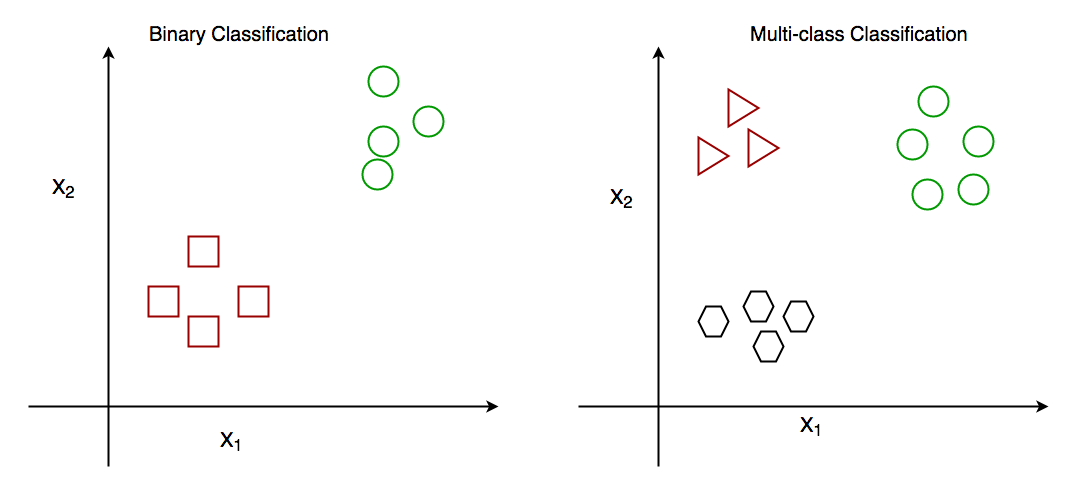
\includegraphics[width=0.9\textwidth]{classification.png}
    \end{figure}
\end{frame}

\begin{frame}{Задача классификации}
    \scriptsize

    \begin{itemize}
        \item Если представить, что мы знаем апостериорное распределение $P(Y = y | \bm{x})$, то не составит труда задать правило $h(\bm{x})$ для предсказания:
        \begin{equation}
            h(\bm{x}) = \text{argmax}_{y \in \mathcal{Y}} P(Y = y | \bm{x}).
        \end{equation}
        \item Распределения неизвестны $\Longrightarrow$ можно оценить с помощью статистических методов
        \item Для пространств большой размерности их оценка затруднена, поэтому чаще используют подход с построением сепарирующей поверхности
        \item  Например, линейный дискриминантный анализ использует линейную функцию для разделения классов
    \end{itemize}

    \vspace{-7pt}

    \begin{figure}[H]
        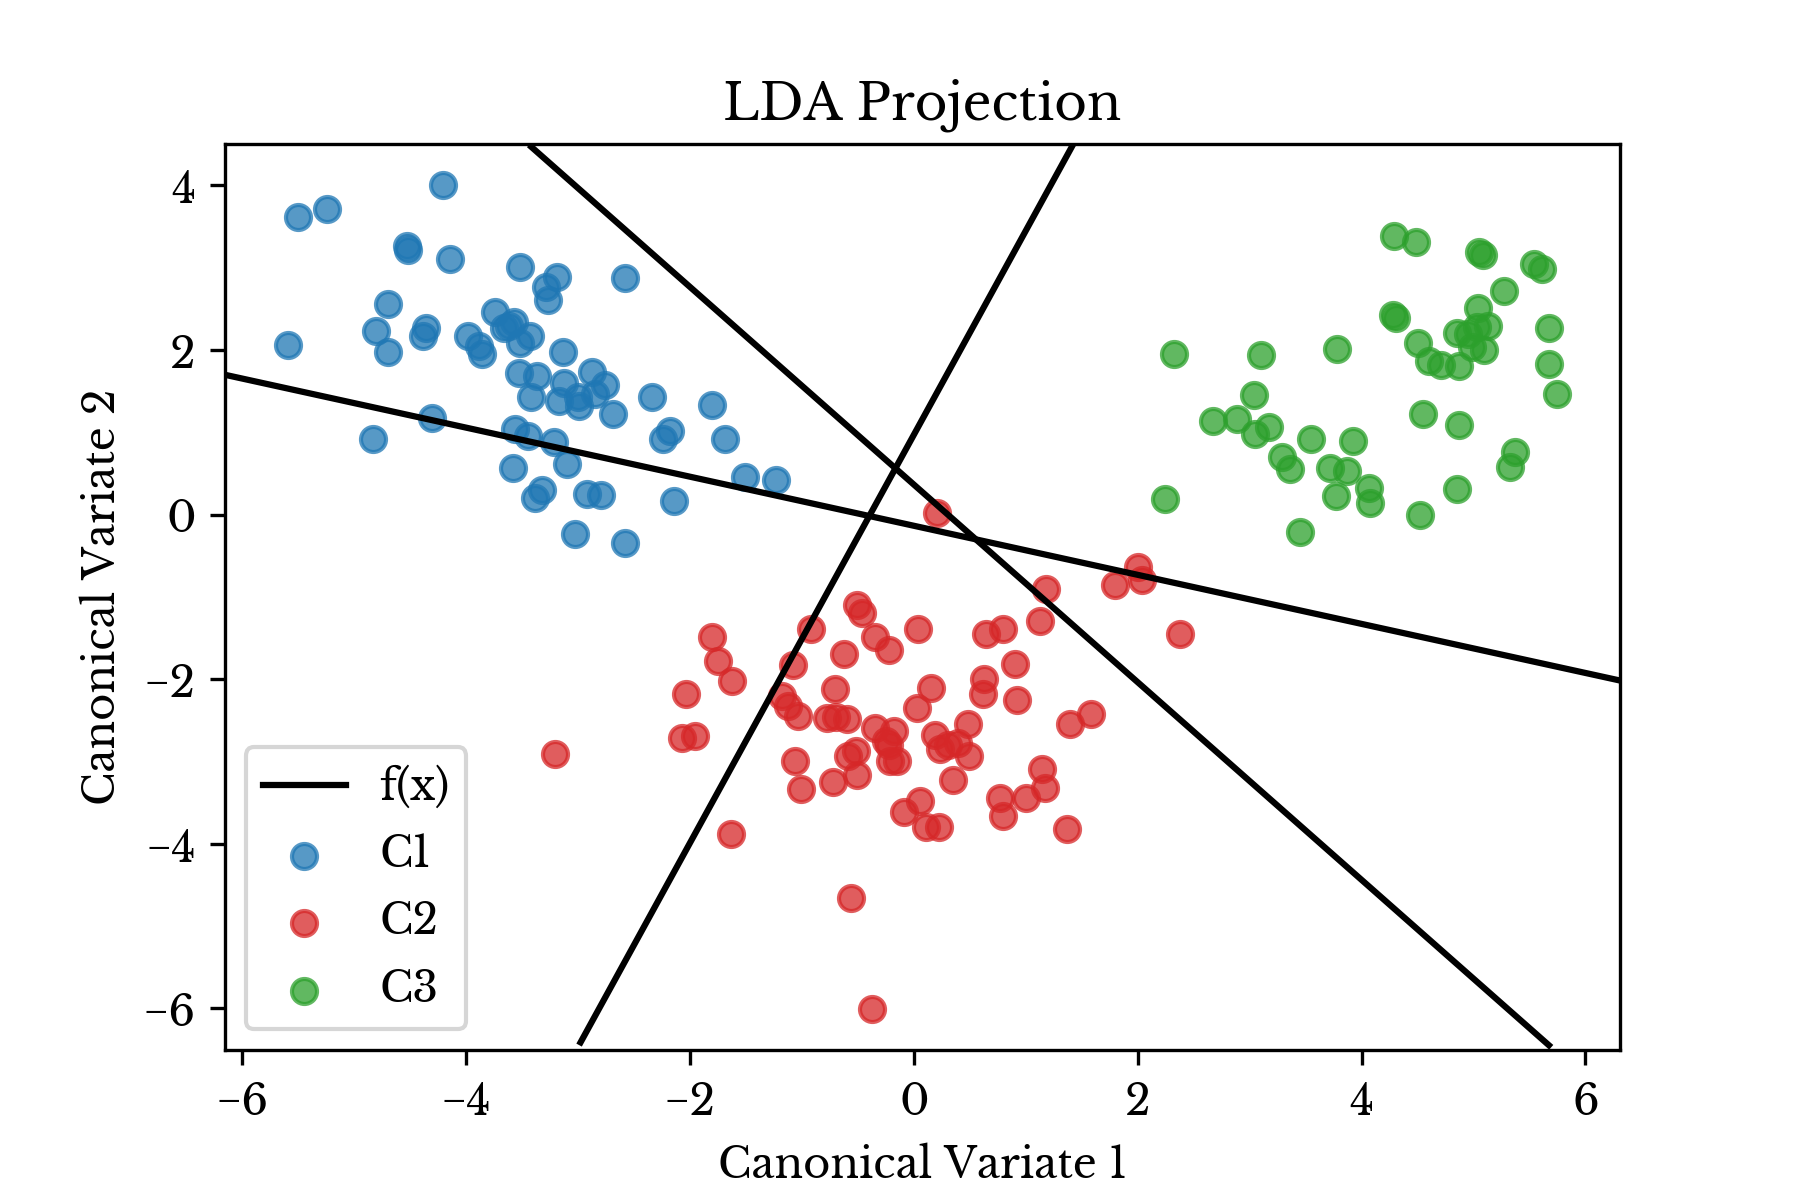
\includegraphics[width=0.7\textwidth]{lda.png}
    \end{figure}

\end{frame}


\begin{frame}{Логистическая регрессия}
    \small

    \begin{itemize}
        \item Логистическая регрессия появляется из желания смоделировать апостериорное распределение линейной функцией, при этом гарантировав, что все вероятности суммируются в единицу и лежат в интервале $[0; 1]$
        \item Это возможно при использовании logit-преобразования:
        \begin{align*}
          \log \frac{P(Y = 1 | X = \bm{x})}{P(Y = K | X = \bm{x})} &= \beta_{10} + \bm{\beta}_1^T \bm{x}, \\
          \log \frac{P(Y = 2 | X = \bm{x})}{P(Y = K | X = \bm{x})} &= \beta_{20} + \bm{\beta}_2^T \bm{x}, \\
          &\dots \\
          \log \frac{P(Y = K - 1 | X = \bm{x})}{P(Y = K | X = \bm{x})} &= \beta_{K-1, 0} + \bm{\beta}_K^T \bm{x}.
        \end{align*}
    \end{itemize}
\end{frame}

\begin{frame}{Логистическая регрессия}
    \small

    \begin{itemize}
        \item Так как сумма вероятностей должна быть равна единице, легко вывести функцию вероятности:
        \begin{align*}
          P(Y = y | X = \bm{x}) &= \frac{exp(\beta_{k0} + \bm{\beta}_k^T \bm{x})}{1 + \sum_{j=1}^{K-1} exp(\beta_{j0} + \bm{\beta}_j^T \bm{x})}, \quad k = 1, \dots, K - 1, \\
          P(Y = K | X = \bm{x}) &= \frac{1}{1 + \sum_{j=1}^{K-1} exp(\beta_{j0} + \bm{\beta}_j^T \bm{x})}.
        \end{align*}
        \item Таким образом, распределение $P(Y = y | X = \bm{x}) = p_y(\bm{x}; \bm{\theta})$ параметризовано $\bm{\theta} = [\beta_{10}, \bm{\beta}_1^T, \dots, \beta_{K-1,0}, \bm{\beta}_{K-1}^T]$
        \item Логарифмическая функция правдоподобия в таком случае имеет вид
        \begin{equation}
            l(\bm{\theta}) = \sum_{i=1}^N \log P(Y = y_i | X = \bm{x}^{(i)}) = \sum_{i=1}^N \log p_{y_i}(\bm{x}^{(i)}; \bm{\theta}).
        \end{equation}
    \end{itemize}
\end{frame}

\begin{frame}{Логистическая регрессия для бинарного случая}
    \footnotesize

    \begin{itemize}
        \item В случае бинарной классификации нам достаточно одной функции для задания распределения. Для удобства заменим класс $2$ на класс $0$. Тогда
        \begin{equation}
            p(\bm{x}; \bm{\theta}) = P(Y = 1 | X = \bm{x}) = \frac{1}{1 + exp(\beta_{0} + \bm{\beta}^T \bm{x})}
        \end{equation}
        так как $P(Y = 0 | X = \bm{x}) = 1 - p(\bm{x}; \bm{\theta})$. Здесь $\bm{\theta} = [\beta_0, \bm{\beta}]^T$
        \item Дополним $\bm{x}$ единицей в начале (смещение). Тогда логарифмическая функция правдоподобия может быть записана как 
        \begin{equation}
        \begin{split}
            l(\bm{\theta}) &= \sum_{i=1}^N \left[ y_i \log p(\bm{x}^{(i)}; \bm{\theta}) + (1 - y_i) \log (1 - p(\bm{x}^{(i)}; \bm{\theta})) \right] \\
            &= \sum_{i=1}^N \left[ y_i \bm{\beta}^T \bm{x}^{(i)} - \log (1 + \exp(\bm{\beta}^T \bm{x}^{(i)})) \right].
        \end{split}
        \end{equation}
        \item Эта целевая функция выпуклая ($\Longrightarrow$ гарантирована сходимость к глобальному максимуму), но нелинейная (требуется метод Ньютона). Частичное доказательство выпуклости: (1) $\bm{\beta}^T \bm{x}^{(i)}$ вогнутая/выпуклая, $\exp$ вогнутая и монотонно возрастающая $\Longrightarrow 1 + \exp(\bm{\beta}^T \bm{x}^{(i)})$ вогнутая; LogSumExp вогнутая, тогда -LogSumExp выпуклая.
        \end{itemize}
\end{frame}

\end{document}
